\chapter{Sunrise III and TuMag: Design and calibration.}

Observing the Sun with the highest possible quality and resolution is crucial for deepening our understanding of the physical processes governing its behavior. This necessity drives the continuous development of new state-of-the-art observatories and advanced instrumentation. Each new instrument or telescope builds upon the technical achievements of its predecessors, integrating past knowledge while introducing innovations that push the boundaries of solar observation. 

An example of such advancements is the third edition of the Sunrise observatory, which marks the culmination of a collaborative effort among several international institutions. Spearheaded by the Max Planck Institute for Solar System Research (MPS) in Göttingen, Germany, the international consortium is also composed by the Spanish Solar Space Consortium (S³PC), the National Astronomical Observatory of Japan (NAOJ), the Kiepenheuer Institute for Solar Physics (KIS) in Freiburg, Germany, and the Johns Hopkins University Applied Physics Laboratory (APL) in the United States. 

Following an initial unsuccessful flight in 2022, which was aborted six hours after launch, Sunrise III was granted a second opportunity in the summer of 2024. On July 10th, 2024, at 04:22:40 UTC, the observatory was successfully launched by the Columbia Scientific Balloon facility (CSBF-NASA) from Esrange, a scientific facility operated by the Swedish Space Corporation in Kiruna, Sweden. After reaching a stable altitude of 37.5 km, the commissioning phase began, marking the official start of the observation campaign. Observations commenced shortly thereafter and continued until the campaign concluded on July 16th at 18:20:54 UTC, when the flight was terminated.

Among the payload instruments aboard Sunrise III, TuMag holds particular significance for this thesis. TuMag, an imaging magnetograph developed by the Spanish Solar Space Consortium (S³PC) under the leadership of the Instituto de Astrofísica de Andalucía (IAA-CSIC) in Granada. The S³PC also includes the Instituto Nacional de Técnica Aeroespacial (INTA), the Instituto de la Riva (IDR-UPM) at the Universidad Politécnica de Madrid, the Universitat de València (UV), and the Instituto de Astrofísica de Canarias (IAC). TuMag is central to this thesis, as the core of the work focuses on its calibration, operations, and data reduction processes.

In this chapter, we present an overview of the Sunrise III mission, with a particular focus on the Tunable Magnetograph (TuMag). We will first outline the scientific motivations behind its development and the design choices. This will be followed by a detailed discussion of the technical specifications of both the mission and TuMag.

\section{Sunrise III}

Equipped with a telescope with a 1m aperture, two slit-based spectropolarimeters and an imaging magnetograph, the Sunrise III observatory is the most complex solar telescope to ever leave the the ground. The coordination of three different scientific insturments allows Sunrise to simultaneously perform narrow-band polarimetric imaging in the visible while carrying out spectropolarimetry in the near-UV and near-IR, from the advantageous point of observation of $\sim$ 36 km of altitude whithout the anoying interference of the atmosphere's turbulence. 

The three instruments aboard Sunrise III have been carefully designed to complement each other and address the scientific purposes of the mission. The Tunable Magnetograph (TuMag, REF), developed by the S³PC, carries out high-spatial-resolution imaging spectropolarimetry in the visible range of light. Able to tune to three different spectral lines, namely the highly Zeeman-sensitive iron lines at 525.02 and 525.06 nm, and the Mg I b$_2$ line, TuMag can probe the photosphere and low chromosphere quasi-simultanously. 

The absence of atmosphere allows the Sunrise Spectropolarimeter and Imager (SUSI, Ref), developed by MPS and NAOJ, to observe in the near-UV, performing imaging and spectropolarimetry in the range of 309-417 nm. The high polarimetric sensitivity and large number of spectral lines present in this range, many of which are sensible to the Hanle effect, allows SUSI to sample many heights in the solar atmosphere at the same time while measuring the weak magnetic fields. 

In the same way that the atmosphere complictaes the observations of the UV range from the ground, observations of many lines in the near-IR are also unfeasable with ground-based instruments due to the telluric contamination of the atmosphere. The Sunrise Chromospheric Infrared spectro-Polarimeter (SCIP, REF), co-developed by NAOJ and IAA-CSIC, takes advantage of the abscence of atmosphere and observes two of the Ca II triplets lines. Spectropolarimetry measurments of these lines provides information of the 3-D structure of the chromosphere and its magnetic fields, derived thanks to the high zeeman sensitivity of the selected lines. Furthermore, the large number of available photons at these wavelengths ensures a high S/N and polarimetric sensitivities. 

The ability to probe simultanously the near-IR, the visible and the near-UV, perfoming high-resolution polarimetric imaging and spectroscopy makes Sunrise III an unique observatory, capable of studying the connection  and interaction of the small-scale phenomena ocurring at different layers of the solar's atmosphere with unprecedented detail and completeness. 

\begin{figure}[t]
    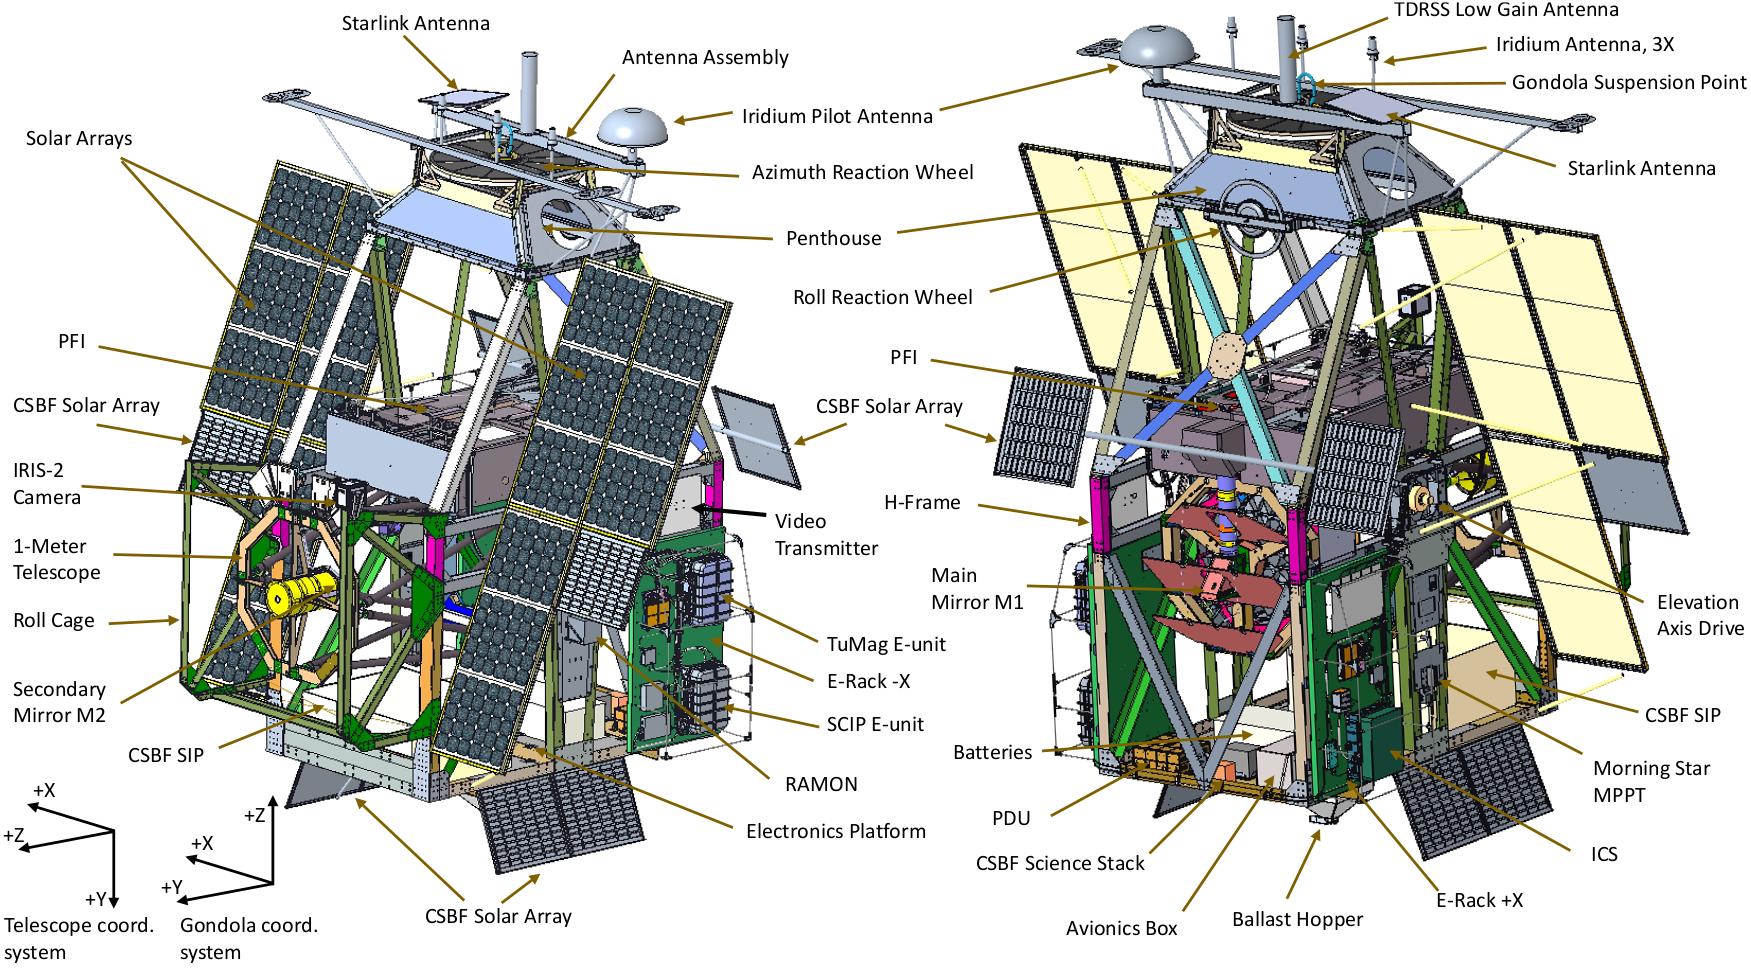
\includegraphics[width=\textwidth]{figures/TuMag/Sunrise_schematic.png}
    \caption{
      Drawing design of the Sunrise III observatory. Image reproduced from XXXXX with permission. \textcolor{red}{No he pedido permiso para esta aún, que es del paper de Sunrise III que mandó Andi, pero creo que quedaría bien algo enseñando el observatorio. Al no estar pulicado el paper de Sunrise no se muy bien cual coger.}}
      \label{fig: SunriseIII}
\end{figure}

\subsection{Observatory's design}

While the scientific instruments are central to the research peformed by Sunrise, several additional subsystems play a crucial role, each contributing to the overall success of the mission.

The structural framework housing all components of the observatory, as well as the interface connecting the observatory to the flight apparatus, is provided by the gondola. This gondola, engineered by APL, is not only tasked with safeguarding the instruments and telescope during ascent and landing, but also with ensuring the stability of the pointing system. Given that the observatory is suspended from a balloon, it is subject to wind-induced motion and pendulum-like oscillations, which threaten the stability required for prolonged observations. The gondola’s pointing control system (PCS) must actively counteract these disturbances in real time by making precise adjustments to the telescope’s elevation and azimuth. In conjunction with the Correlating Wavefront Sensor (CWS), developed by KIS, which is responsible for image stabilization and autofocus, the PCS was required to achieve a pointing accuracy better than 0.005" root mean square (rms) over extended periods to facilitate long-duration observations.

The Sunrise III telescope is a Gregory-type reflector with a 1-meter aperture, featuring a 234 mm central obscuration and an effective focal length of 24.2 meters. This configuration provides a field of view (FoV) of 3.4', corresponding to approximately 150 Mm on the solar surface. The telescope directs light to the post-focus instrumentation platform (PFI), located above the telescope. The PFI houses the three scientific instruments and the CWS, and is responsible for distributing light among these four instruments. This distribution, performed by the Image Stabilization and Light Distribution Unit (ISLiD), must efficiently separate the different wavelengths in a photon-efficient manner to provide the highest number of available photons to each instrument. 

While all the subsystems discussed thus far directly influence the optical performance, it is equally important to recognize the crucial role played by other subsystems, such as the electronics and software control. In particular, the Instrument Control System (ICS) is responsible for the management of the observatory, gathering housekeeping and issuing commands to the electronic units of each instrument. As will be elaborated in the following chapter, Sunrise III observations were designed to operate in a semi-autonomous manner through the use of pre-programmed timelines. This approach requires that all electronic systems function in synchrony, with minimal human intervention. 

\subsection{Science with Sunrise.}

The absence of Earth's atmosphere opens the window for IR and UV observations and offers a level of image stability that cannot be achieved in ground-based observatories due to atmospheric seeing. However, these advantages are also present in spaceborne missions, such as the Spectro-Polarimeter and Narrowband Filter Imager aboard the Solar Optical Telescope of the Hinode mission (\citealt{Hinode}, \citealt{sot}), or the Polarimetric and Helioseismic Imager aboard Solar Orbiter (SO-PHI) (\citealt{PHI}, \citealt{SO}), among many others. Nonetheless, spaceborne missions have strong restrictions regarding payload, mass and data rate. 

The abscence of these restrictions in balloon-borne observatories allows for a more complex and versatile instrumentation than the one present in space missions. The combination of these two factors, namely the absence of atmosphere and the complex and advanced instrumentation they can carry, places observatories such as Sunrise in an unique position, and provides them with unique presepectives on solar phenomena.

Many aspects of the physical processes driving our Sun remain unresolved. The mechanisms underlying various solar phenomena are still the subject of debate, ranging from the origin and removal of magnetic flux in the solar photosphere to the processes responsible for heating the chromosphere and corona, as well as the small-scale dynamics of solar plasma. The three instruments aboard Sunrise work in consonance to provide novel insights into these phenomena, and aim at helping the community solve some of the open questions of solar physics. 

The magnetic field, present across multiple scales and heights, is the principal driver of solar activity. Understanding the magnetic field is essential for comprehending the processes that govern solar phenomena, energy distribution, and plasma dynamics. Numerous works direct their efforts to the study of the structures and evolution of magnetic fields. For instance, several works study  the emergence of magnetic flux in the photosphere, such as, \cite{flux_emergence_1} and \cite{flux_emergence_2}, where they utilized Sunrise I IMaX data to examine small-scale flux emergence events occurring within solar granules. Likewise, the processes responsible for magnetic flux removal are not fully known. Several studies, such as \cite{flux_removal_1} and \cite{flux_emergence_2}, have proposed mechanisms for flux removal in the photosphere; however, no model is favoured over the other by current observations.

A thorough 3-dimensional analysis of the magnetic fields is essential to study these events. The combination of spectropolarimeters and vector magnetographs aboard Sunrise, which are capable of measuring strong magnetic fields through the Zeeman effect, and detecting weaker, more turbulent \citep{quiet_sun_living_review} magnetic fields using the Hanle effect - particularly sensible in the UV - can provide a new and complete perspective of these events.  

One of the scientific targets of Sunrise is the study of the upper atmosphere, whose dynamics and heating mechanisms are not yet completely understood. In fact, the transfer of energy from the lower layers to the chromosphere and corona is one of the open problems in stellar astrophysics. Several studies propose mechanisms in which the magnetic field plays a central role in this energy transfer. Some works suggest upward currents generated by the slow motion of plasma in the photosphere as a driving mechanism (\cite{upwards1}, \cite{upwards2}), while others highlight heating processes induced by jets \citep{jetscorona} or magnetic vortex phenomena, such as twisted magnetic fields known as solar tornadoes \citep{solar_tornadoes}.

Although some observational signatures of these processes have been detected, the detailed characterization of these events requires higher spatial and temporal resolutions than those currently available. The high-cadence UV observations, where several spectral lines sensitive to the weaker magnetic fields of the chromosphere are present, combined with magnetic field maps of the photosphere and lower chromosphere provided by TuMag, and complementary observations of the Ca II infrared lines, provide Sunrise with the necessary tools to investigate these phenomena with unprecedented detail.

Sunrise also aims to provide novel insights into small-scale plasma dynamics. The Sun is highly dynamic, with structures evolving on timescales of minutes. Several studies propose that the magnetism in the quiet Sun is driven by the turbulent small-scale dynamics of the plasma (\cite{small_scale_dynamo}, \cite{small_scale_dynamo_2}, \cite{small_scale_dynamo_3}, among others). However, investigating these processes requires high spatial and temporal resolutions, which are often unattainable in ground-based observations. Similarly, other approaches to plasma dynamics, such as helioseismology \citep{helioseismology}, also demand such high-resolution data. To address these challenges, Sunrise III conducted extended, highly stable due tothe abscence of atmospheric seeing, and uninterrupted observations lasting up to 6 hours, with the highest temporal resolution permitted by the (S/N) requirements.

In addition to these objectives, Sunrise will explore new and exciting areas, including the measurement of the polarized solar spectrum in the UV. This spectral region remains largely unexplored due to the technical challenges associated with its observation. Atmospheric absorption makes it impossible to observe this band from ground-based observatories, and it has yet to be measured by any space mission. SUSI is the first UV spectropolarimeter to acquire high-resolution data in this wavelength range.

\section{The Tunable magnetograph: TuMag}

\begin{table}
    \centering
   \begin{tabular}{cc}
    \hline
    \hline
    Requirements & Value \\
    \hline
    Field of view & $63''$ x $63''$ \\
    RMS wavefront error & $W \sim \lambda / 14$\\
    Spatial sampling & $3 \times 3 $ pixels \\
    Plate scale & $0.0378''$ / pixel \\
    Polarimetric efficiencies & $\epsilon _ {1, 2, 3} \lessapprox \frac{1}{\sqrt{3}}$\\
    SNR ratio & $\left(\frac{S}{N}\right) _ 0 \gtrapprox 1700$ \\
    Spectral resolution & $< 9$ pm\\  
    Spectral lines & Fe I 5250.2 \r{A}, Fe I 5250.6 \r{A} and Mg I $b_2$ 5172.7 \r{A}. \\
    Time for a two-line observation & $< 90$ s\\
    \hline
    \hline
    \end{tabular}
    \caption{Tumag scientific requirements.}
    \label{table: Tumags requirements}
\end{table}

TuMag is an FPI-based tunable imaging spectropolarimeter, capable of measuring the full Stokes vector across various spectral lines. This tunability allows TuMag to probe the magnetic field in both the photosphere and lower chromosphere, with high resolving power, thanks to its near-diffraction-limited imaging capabilities. The design of TuMag is inherited from IMaX, the imaging spectropolarimeter that flew aboard previous Sunrise missions. However, TuMag incorporates several advancements over its predecessor, including the addition of filter wheels for tunability between spectral modes and calibration systems, along with newly designed cameras and modulation packages.

In this section, we present an overview of the design of TuMag  and its performance. It is important to note that this discussion will primarily focus on the instrument's optical design and performance—specifically its polarimetric, spectral, and imaging properties. The thermal design and control software, while crucial to the instrument’s functionality, will not be covered here to avoid excessive length. Nonetheless, it is essential to acknowledge that these aspects are integral to TuMag’s overall performance and represent a substantial portion of the effort contributing to its success.

\subsection{TuMag's design and light path.}

As a polarimeter, TuMag must be able to measure the full Stokes vector of the incoming light. To achieve this, it must generate four distinct modulation states and measure them in an almost simultaneously manner. As a spectrometer, TuMag must possess the capability to select specific wavelengths along multiple spectral lines. This selection process involves, first filtering the light with a pre-filter, which selects a "broad" spectral range, followed by an etalon that further narrows the bandpass within the selected range. Throughout this procedure, stringent requirements regarding polarimetric sensitivity (efficiency), spectral resolution, and imaging quality must be maintained. A summary of these requirements is presented in Table \ref{table: Tumags requirements}.

\begin{figure}[t]
    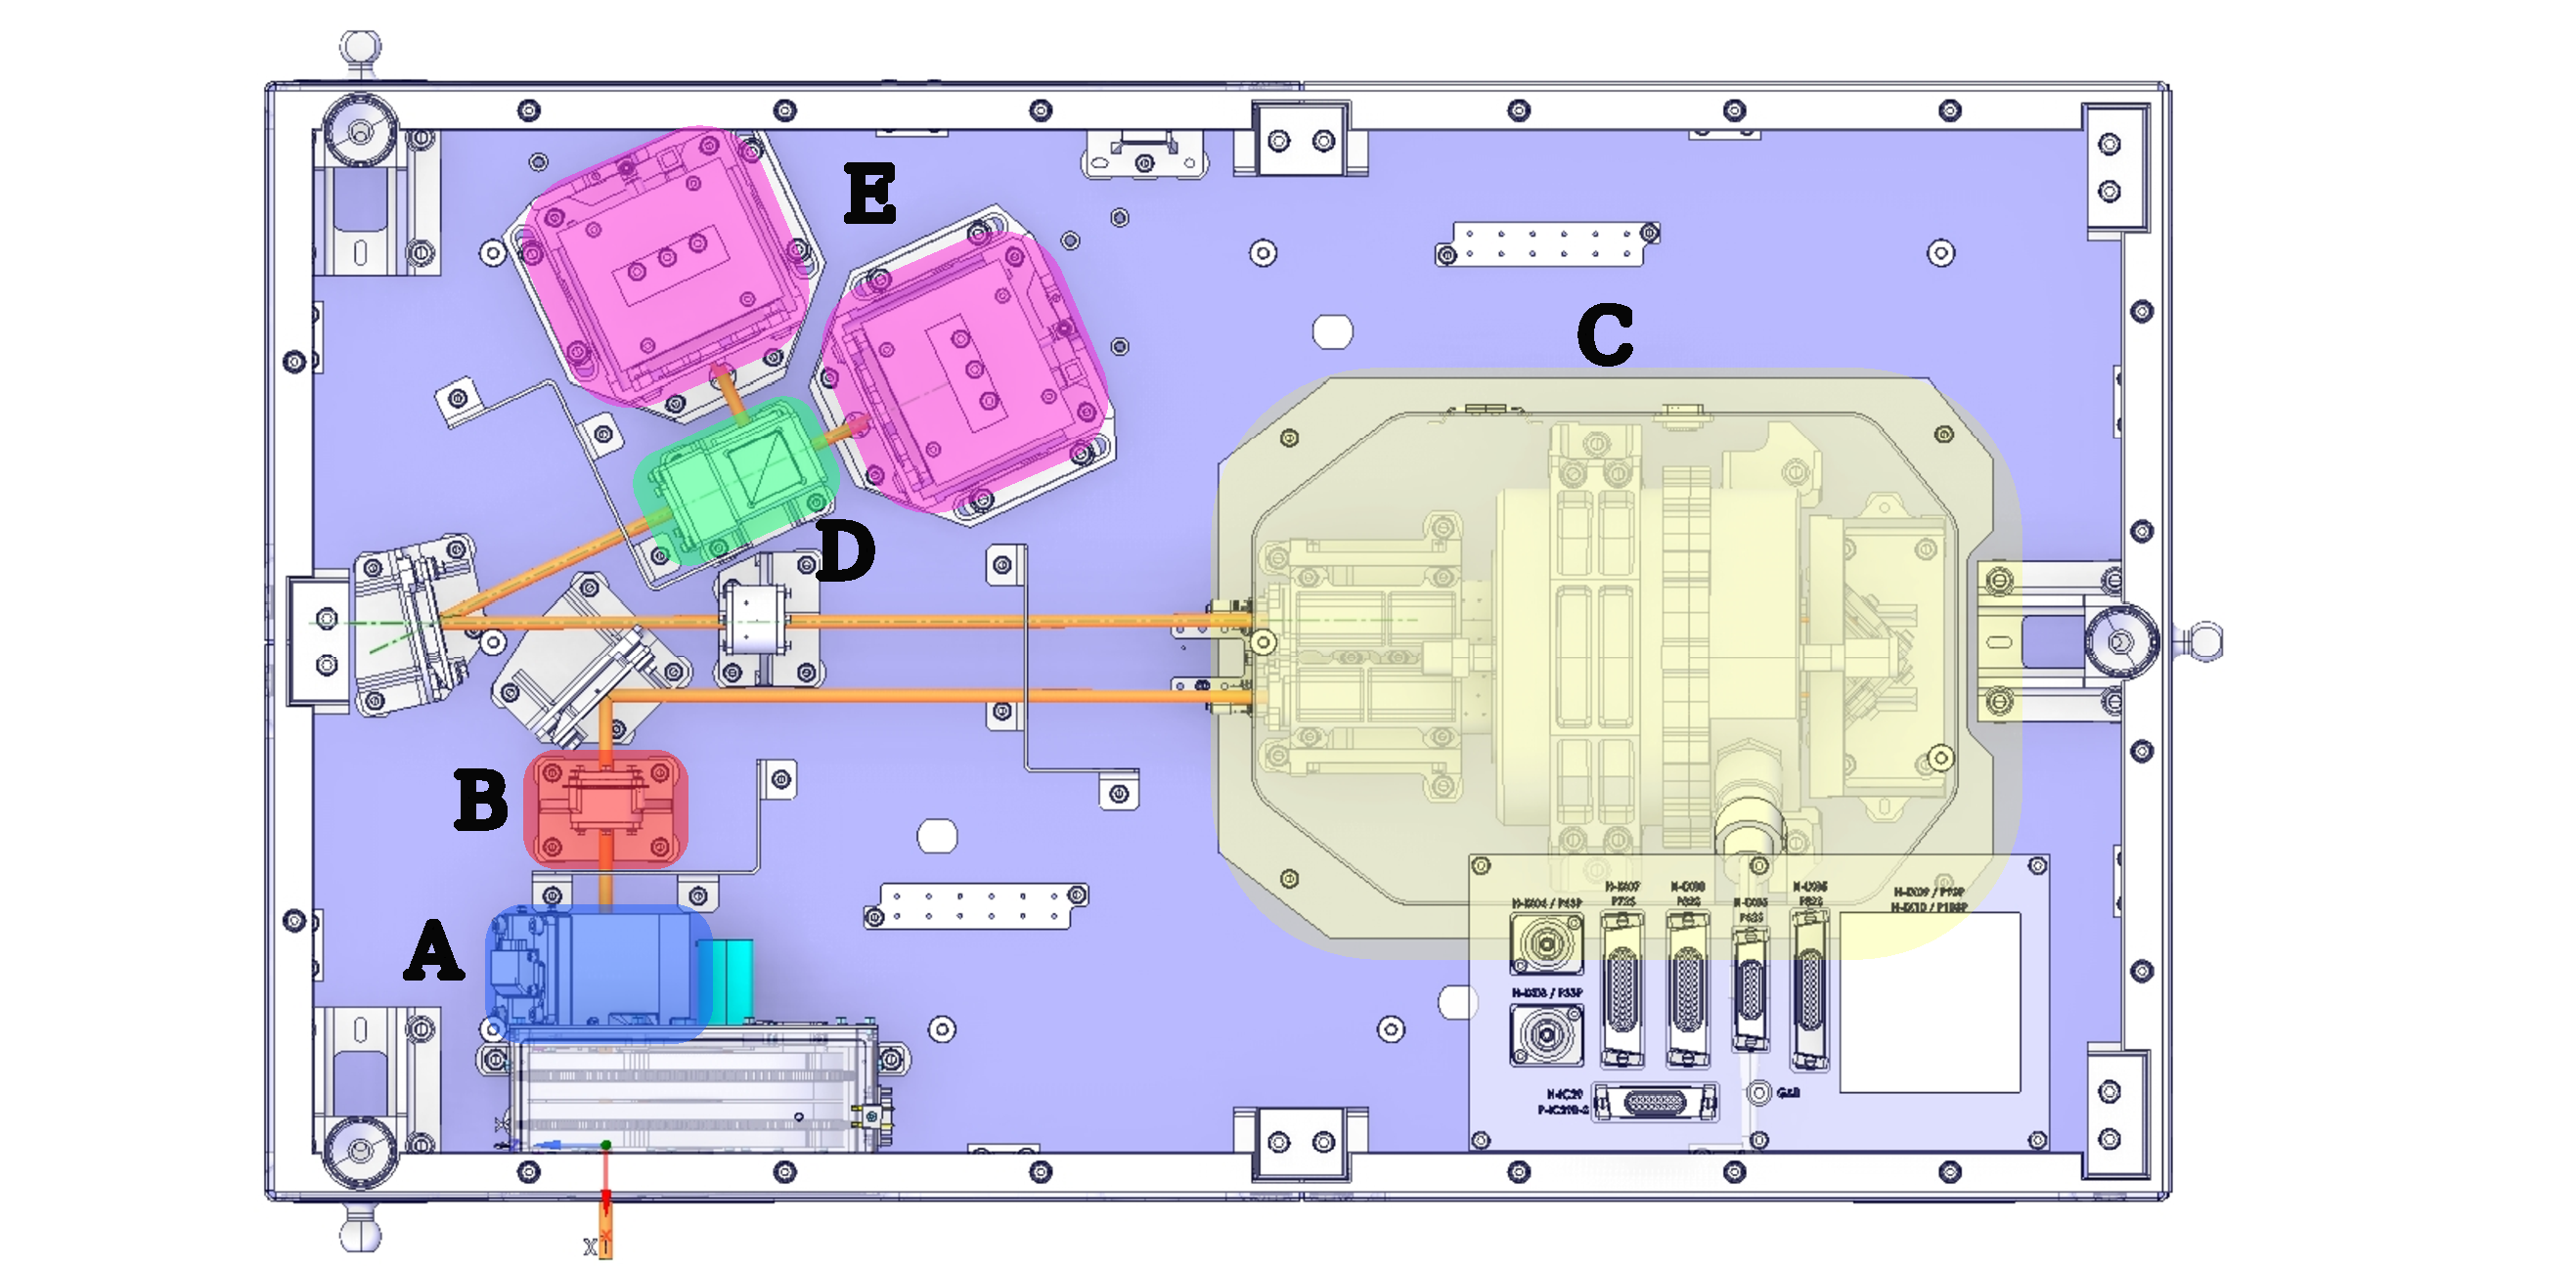
\includegraphics[width=\textwidth]{figures/TuMag/Scheme.pdf}
    \caption{Schematic representation of the Tumag instrument. Some relevant optical devices in the light path (yellow line) are highlighted with a colored box and labeled with leters from A to E: A) Filter wheel, B) PMP, C) Etalon oven, D) beam-splitter and E) cameras. Image taken from TUMAG PAPER REF, reproduced with permission.      
    \label{fig_tumag:scheme}}
\end{figure}

Light is delivered to TuMag by the ISLiD system and subsequently re-imaged onto two cameras where the images are recorded. Before reaching the cameras, the light passes through all the different subsystems of the optical unit. The first components encountered by the light are a blocking prefilter and the filter wheels (box A in Fig. ~\ref{fig_tumag:scheme}). The blocking prefilter, with a wide bandpass centered at 520 nm, is employed to eliminate unwanted spectral ranges. The filter wheels  are comprised by a double-disk system \citep{filter-wheels} that houses the prefilters for selecting specific spectral lines and a series of calibration modules. Specifically, three prefilters are mounted on the second disk of the filter wheel, corresponding to the spectral lines Fe I 5250.2 \r{A}, Fe I 5250.6 \r{A}, and Mg I $b_2$ 5172.7 \r{A}. Additionally, the filter wheels include a PD plate, which is used to introduce a known defocus into the final image to facilitate image reconstruction techniques, along with a linear polarizer, a plate of micropolarizers, and a pinhole set, employed during calibration observations.

After passing through the filter wheels, the light is directed into the Polarization Modulation Package (PMP), a subsystem derived from the SO/PHI instrument (\citealt{pmp1}, \citealt{PHI}), highlighted with the red box in Fig.\ref{fig_tumag:scheme}. The PMP's primary function is to modulate the light to produce the different polarization states required to deduce the Stokes components. This is achieved using two liquid crystal variable retarders (LCVRs), which are oriented with their fast axes at 45$^\circ$ relative to each other. These LCVRs induce a retardance on the transmitted light that varies with the voltage applied across the crystals. The system can operate in two distinct modulation schemes: a vector modulation scheme, which generates four independent linear combinations of equally-weighted Stokes components across consecutive observations, allowing for the retrieval of the full Stokes vector after demodulation; and a longitudinal modulation scheme, which generates only two modulations, providing information solely on the intensity and circular polarization.

Following modulation, the light is directed into a LiNbO$_3$ Fabry-Pérot etalon, highlighted in yellow in Fig.\ref{fig_tumag:scheme} (box C). Likewise IMaX, the etalon operates in a collimated setup and with a double pass configuration \citep{etalon-doublepass}. In this configuration, after the light passes through the etalon once, it is redirected by a pair of mirrors to pass through the etalon a second time. This double-pass configuration significantly enhances spectral resolution by narrowing the transmission profile. The LiNbO$_3$ etalon tunes the resonance wavelength by varying the refractive index of the cavity through the application of high voltages (ranging from $-4000$ V to $4000$ V). Compared to air-gapped etalons, these kind of etalons offer the advantage of having no moving parts, which is particularly beneficial for spaceborne or balloon-borne instruments. However, this advantage comes with the need for precautions to prevent discharges caused by air ionization.

The final optical element the light encounters before reaching the cameras is a polarizing beam splitter (green box C in Fig.\ref{fig_tumag:scheme}). At this stage, the light beam is divided into two orthogonal, linearly polarized components, each directed towards a different camera. This dual-beam configuration \citep{lites-doublebeam} is designed to minimize spurious signals induced by jitter of the gondola (see \cite{libro_JoseCarlos} for an extended discussion), as it effectively cancels fluctuations from Stokes I to the other Stokes parameters that may arise due to image motion or solar evolution (\textit{i.e.} cross-talk).

Light then reaches the cameras, shown with pink boxes (boxes E) in the scheme, where images from both are recorded and stored. After mission recovery, the data is processed on-ground to combine images from the different cameras, modulation states, and spectral lines, ultimately deriving the scientific products. This processing and reduction of the data is accomplished using software specifically developed for TuMag, which will be extensively discussed in Chapter \ref{CH:Pipeline}. 

\subsection{Instrument performance and verification.}

All subsystems within the TuMag light path function collaboratively to deliver high-resolution spectroscopic data of the solar spectrum. To ensure data quality, TuMag underwent multiple verification and calibration processes, during which its spectral, polarimetric, and imaging properties were meticulously tested. These procedures, commonly referred to as end-to-end (E2E) calibration tests (see \cite{e2e-tests-inta} for a detailed description of the tests), were conducted at various stages of the mission. Specifically, they were performed during the assembly, integration, and verification (AIV) activities with the stand-alone instrument at INTA facilities in Madrid, Spain; during the AIV phase of the PFI platform at MPS facilities in Göttingen, Germany; and during the TuMag AIV phase in the Sunrise III mission at ESRANGE facilities in Kiruna, Sweden. These tests were designed not only to validate the instrument's capabilities but also to measure critical parameters such as the tuning constant of the etalon, modulation matrices, and best-focus position—each of which is vital for the optimal operation of TuMag and the subsequent data processing. We will now delve into the details of the imaging, spectral and polarimetric properties of the instrument as well as the verification processes and results, as the two are intimately related.  

\subsubsection{Imaging performance.}
TuMag captures photons using two custom-made cameras \citep{tumag-cams} equipped with GPIXEL back-illuminated GSENSE400BSI detectors, each featuring a $2k \times 2k$ pixel array, and specifically designed to meet TuMag's scientific requirements. These cameras provide a broad FoV of $63'' \times 63''$, sufficient to encompass an entire medium-sized active region, with a plate scale of $0.0378''$/pixel.

In order to fulfill the requirement of the wavefront error of $W \sim \lambda / 14$, the instrument must have means to correct for the additional aberrations introduced by the telescope, the image stabilization and light distribution (ISLiD) system and uncorrected jittering. For this purpose, TuMag is equipped with a PD plate in the filter wheel that allows for the assesment of the PSF during the observations to apply image restoration techniques during the data processing.  

The imaging E2E tests involved projecting several targets at the F4 focus, including a USAF test target, star targets, and a grid, observed both with and without the PD plate. These targets were utilized to evaluate the MTF and to assess the resolving power of TuMag. The PD measurements enabled verification of the wavefront error (WFE) derived from the MTF and an evaluation of the image quality following image restoration. 

The USAF target \footnote{The 1951 USAF target from Thorlabs Inc, model: R1DS1N.} consists on a series of horizontal and vertical line pairs (lp) aranged in sets of three with varying resolutions. Identifying the highest resolution group observable with TuMag allows for a fast diagnostic of the instrument resolution and performance. In fig.~\ref{tumag : USAF}, measurements of group 4 and 5 (and higher) of the USAF target are shown for both cameras and the three pre-filters. The second set of group 5 (highlighted in a white box), which corresponds to 35.9 lp/mm in the target and 24.3 lp/mm in the image, is of special interest since its close to the Airy disk radius (26.4 lp/mm) and therefore close to TuMag's resolution limit. 

\begin{figure}[t]
    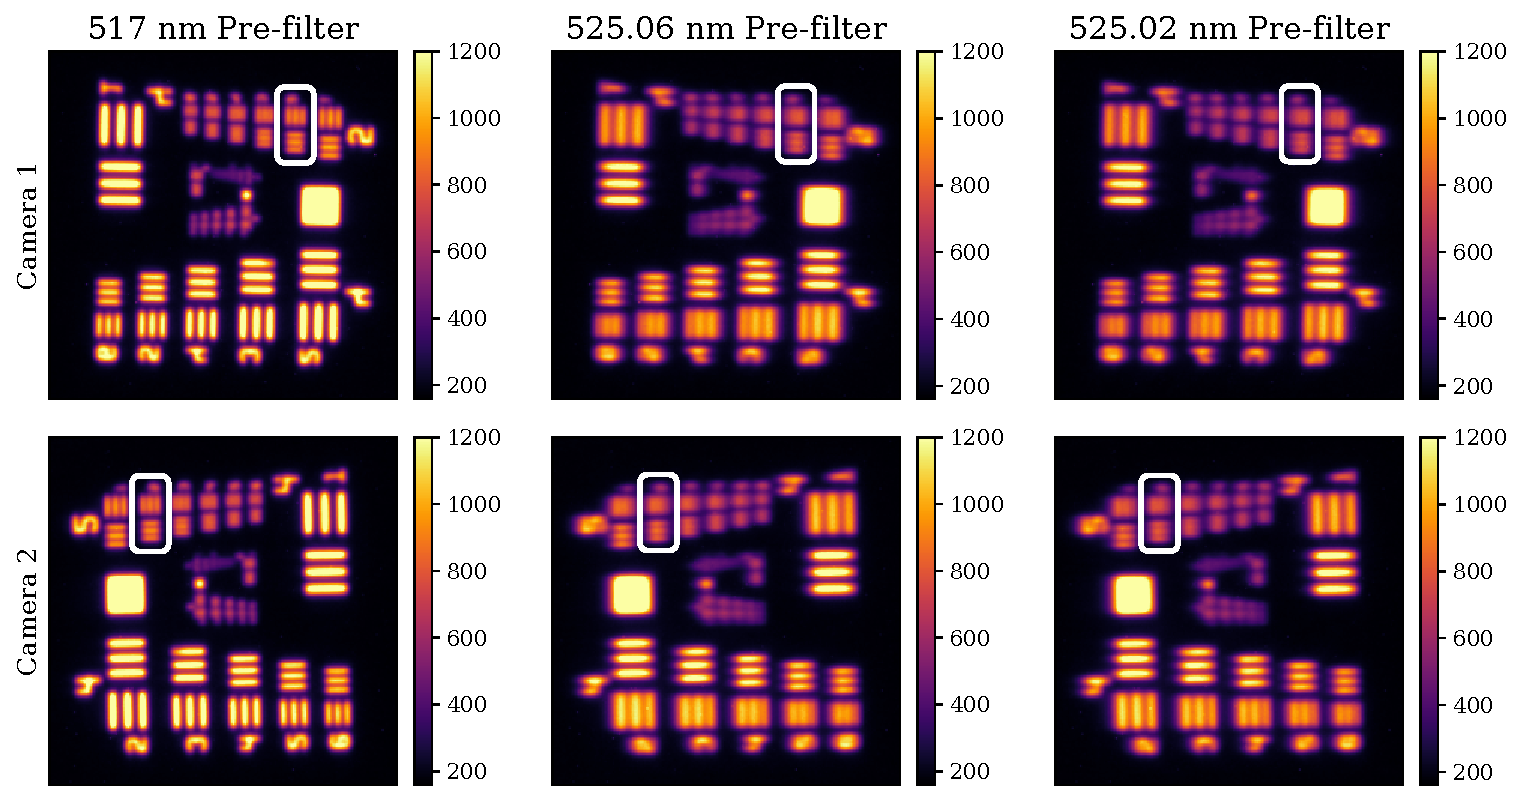
\includegraphics[width=\textwidth]{figures/TuMag/USAF_E2E.pdf}
    \caption{
      USAF target measurements for both cameras and the three pre-filters performed during E2E tests at INTA facilities on December 2021. The white boxes highlight the second element of the test group 5 (35.9 lp/mm). The scale of the images is set in digital counts.}
      \label{tumag : USAF}
\end{figure}

The results show a better optical performance for the 517 nm pre-filter than the other two pre-filters. The USAF 5.2 set is clearly resolved fo this pre-filter in both cameras showing almost no differene between vertical and horizontal resolutions. However, results for the 525 nm prefilters exhibit a worsening of the resolution, with the same set being hardly resolved in the horizontal direction in both prefilters. 

\begin{figure}[t]
    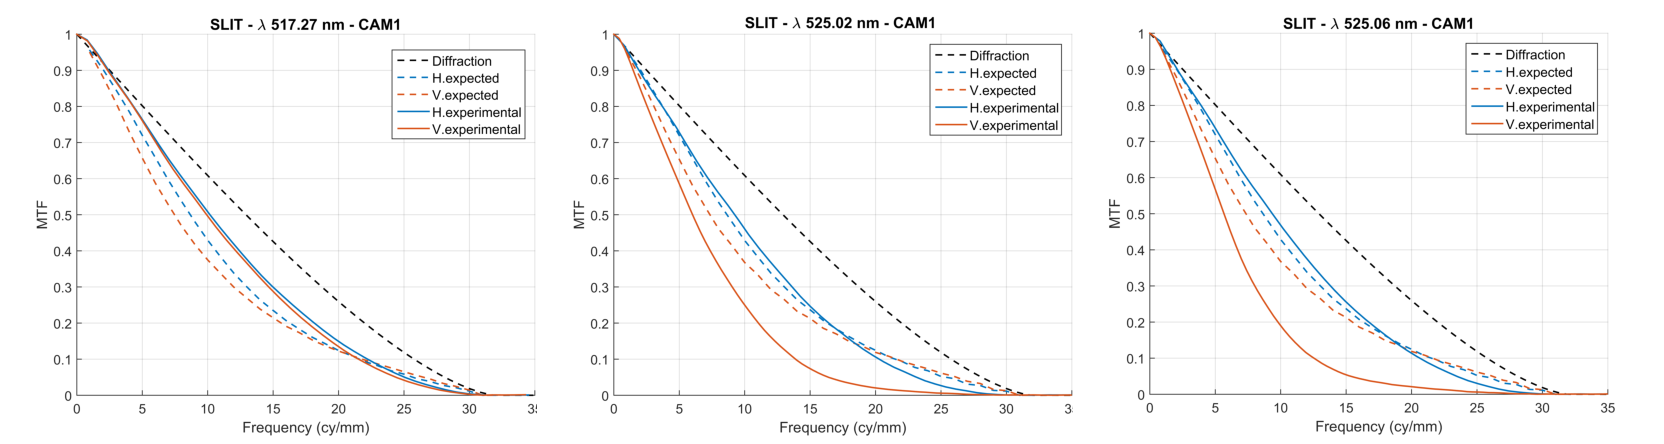
\includegraphics[width=\textwidth]{figures/TuMag/mtfs.pdf}
    \caption{MTFs derived for camera 1 (very similar results for camera 2) for the three pre-filters from measurements of the stand-alone AIV phase performed at INTA in December 2021.  
      \label{fig_tumag:mtfs}}
\end{figure}


However, a more precise evaluation of the optical performance can be achieved from the MTFs. Figure \ref{fig_tumag:mtfs} shows the MTFs computed with a slit target (see \cite{slanted-method} for a description of the MTF computation method) during the E2E tests performed in December 2021 at INTA facilities. These results agree with the diagnostic carried with the USAF tests: the 517 nm pre-filter shows a good performance in both directions, with values above the expected behaviour. Meanwhile, 525 pre-flters exhibit a large difference between different directions with an important drop in vertical resolution in both cases. This observed astigmatism is attributed to the etalon and physical deformations of the pre-filters caused by the mechanical method used to secure and tilt them. This effect is particularly noticeable in the iron pre-filters due to the higher angles of incidence required for their tuning.

\begin{table}[t]
    \centering
   \begin{tabular}{ccccc}
    \hline
    \hline
    Pre-filter and & Strehl ratio & Strehl ratio & WFE& WFE\\
    camera & Vertical & Horizontal & Vertical & Horizontal\\
    \hline
    517 nm - Cam 1 & 0.782 & 0.826 & $\lambda/12.7$ & $\lambda/14.5$ \\
    517 nm - Cam 2 & 0.761 & 0.806 & $\lambda/12.1$ & $\lambda/13.5$ \\
    525.02 nm - Cam 1 & 0.436 & 0.725 & $\lambda/6.9$ & $\lambda/11.1$ \\
    525.02 nm - Cam 2 & 0.405 & 0.726 & $\lambda/6.6$ & $\lambda/11.1$ \\
    525.06 nm - Cam 1 & 0.451 & 0.764 & $\lambda/7$ & $\lambda/12.1$ \\
    525.06 nm - Cam 2 & 0.444 & 0.736 & $\lambda/7$ & $\lambda/11.3$ \\
    \hline
    \hline
    \end{tabular}
    \caption{Optical performance evaluated from the MTFs obtained with the slit target at December 2021 E2E tests.}
    \label{table: Optical-performance}
\end{table}


The comparison of the obtained MTF and the difraction-limited one allows for an estimation of the Strehl ratio, and consequently the wavefront error (see section \ref{sec: intro-imaging}).

Table \ref{table: Optical-performance} shows the results for the Strehl ratios and WFE derived from this computation. All values, except for the horizontal resolution in camera 1 of the 517 nm prefiter are lower than the $\lambda/14$ set as a requirement. However, images can always be restored if $WFE \gtrapprox \lambda / 5$ \citep{restoration-limit} if the PSF is known, thus the need for the inclusion of PD capabilities in the instrument. Furthermore, PD techniques not only allow us to enhance the optical performance of the instrument but also evaluate the optical performance during the calibrations in order to verify the results obtained through the computation of the MTF. 

\begin{figure}[t]
    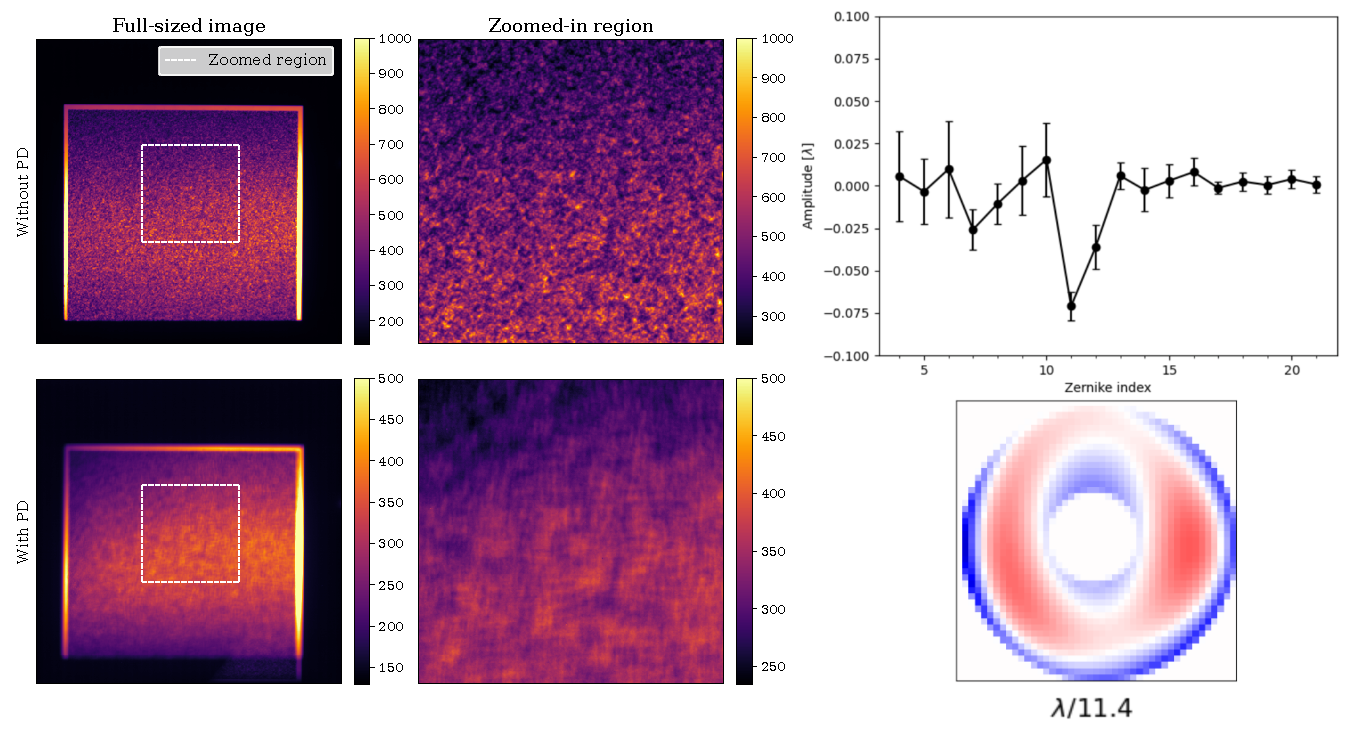
\includegraphics[width=\textwidth]{figures/TuMag/PD_e2e.pdf}
    \caption{Random dot target measurements of the 517 nm pre-filter with the camera 1 and without the PD plate (left and central columns) taken during the Sunrise III AIV phase in Kiruna on April 2024. The right column shows the Zernike coefficients obtained from the PD analysis in the top panel and the 2D representation of the rms WFE. The PD analysis has been carried out by F. J. Bailén, reproduced with permission.}
      \label{tumag : PD}
\end{figure}

Figure \ref{tumag : PD} shows the measurements and results of the PD analysis for the 517 nm pre-filter and the camera 1. The measurments were carried out during the final E2E tests performed at Kiruna on April 2024 using the random dot target (left and central columns of the figure). The measurements consist on 5 sets of focused-defocused pairs of images. The PD algorithm is run over a zoomed-in region of 600 pixels in sub-patches of 128x128 pixels. The mean Zernike coefficients are shown in the top right panel, where the error has been computed as the standard deviation between different sub-patches. A 2D representation of the rms WFE is also shown in the bottom right panel. 

The PD analysis indicates a small amplitude for most aberrations, with coefficients beyond Z15 approaching zero, except for the spherical aberration ($Z_{11}$, $Z_4 ^0$) which is the dominant contribution to the rms wfe. However, the results exhibit significant dispersion, as reflected by error bars that reach values up to 0.025$\lambda$ for the first coefficients. Both the defocus and astigmatism are pretty low (Zernike indexes 4, 5 and 6, $Z _ 2 ^0$, $Z _ 2 ^{-2}$ and $Z _ 2 ^2$, respectively), agreeing with the results obtained from the MTF analysis which showed a good resolution in both vertical and horizontal directions. The overall rms WFE obtained from this analysis is $\lambda / 11.4$. It is important to note that the PD analysis shown here was carried out at the final stages of the calibration campaign, with TuMag mounted on the PFI and the with the light being fed to the instrument through the telescope and ISLiD system, whereas the MTF determination was conducted in the stand-alone AIV phase, without the aberrations introduced by these systems. Nevertheless, both analyses agree on a WFE better than $\lambda / 10$, indicating very high optical quality, despite the fact that the FPI of TuMag operates in a collimated configuration, which is known to degrade optical performance \citep{ghosts-etalon}.

\subsubsection{Spectral performance.}

TuMag filters wavelengths through a sequential process, beginning with a broad blocking pre-filter that eliminates unwanted regions of the solar spectrum, and followed by a second narrow-band pre-filter that is tuned to the three selected spectral lines. Finally, the LiNbO$_3$ Fabry-Pérot etalon is encharged of selecting a very narrow band around specific wavelengths along the spectral lines. The narrow-band pre-filter and the etalon are critical to TuMag's spectroscopic performance and require careful evaluation during calibration.

The three TuMag pre-filters were custom-manufactured by Materion$^{TM}$ and have a full width at half maximum (FWHM) close to 1 nm. They are centered near the rest wavelength of the three spectral lines at normal incidence, with a peak transmission exceeding 80\% in all cases. Each pre-filter was tuned by adjusting the incidence angle to align the peak transmission wavelength with the spectral line core. This process was performed using a coelostat at the INTA facilities, where the rest positions in volts of the spectral lines were determined. The Fe I 5250.2 \r{A} line was found at 2129 V, the Fe I 5250.6 \r{A} line at -2507 V, and the Mg I $b_2$ 5172.7 \r{A} line at -2245 V. While this tuning was successful, particularly for the iron lines, the spectral position of the pre-filters was found to be highly sensitive to illumination conditions. This sensitivity was evident from the shifts observed in the pre-filter measurements during the various stages of the assembly process. As illustrated in the left column of Fig.~\ref{fig_tumag: spectroscopic_results}, the variation in the spectral position of the pre-filters is not sufficient to cause the spectral line to be blocked by the pre-filter, but it may result in the spectral line falling on the wing of the pre-filter during observations.

\begin{table}
    \centering
   \begin{tabular}{cc}
    \hline
    \hline
    Property & Value \\
    \hline
    Reflectivity & 0.892 \\
    Thickness & 281 $\mu$m\\
    FWHM (double-pass) & 0.8\\
    Tuning Constant & 3300 V/\r{A}\\
    \hline
    \hline
    \end{tabular}
    \caption{Tumag Fabry-Pérot specifications.}
    \label{table: Tumags etalon}
\end{table}

\begin{figure}
    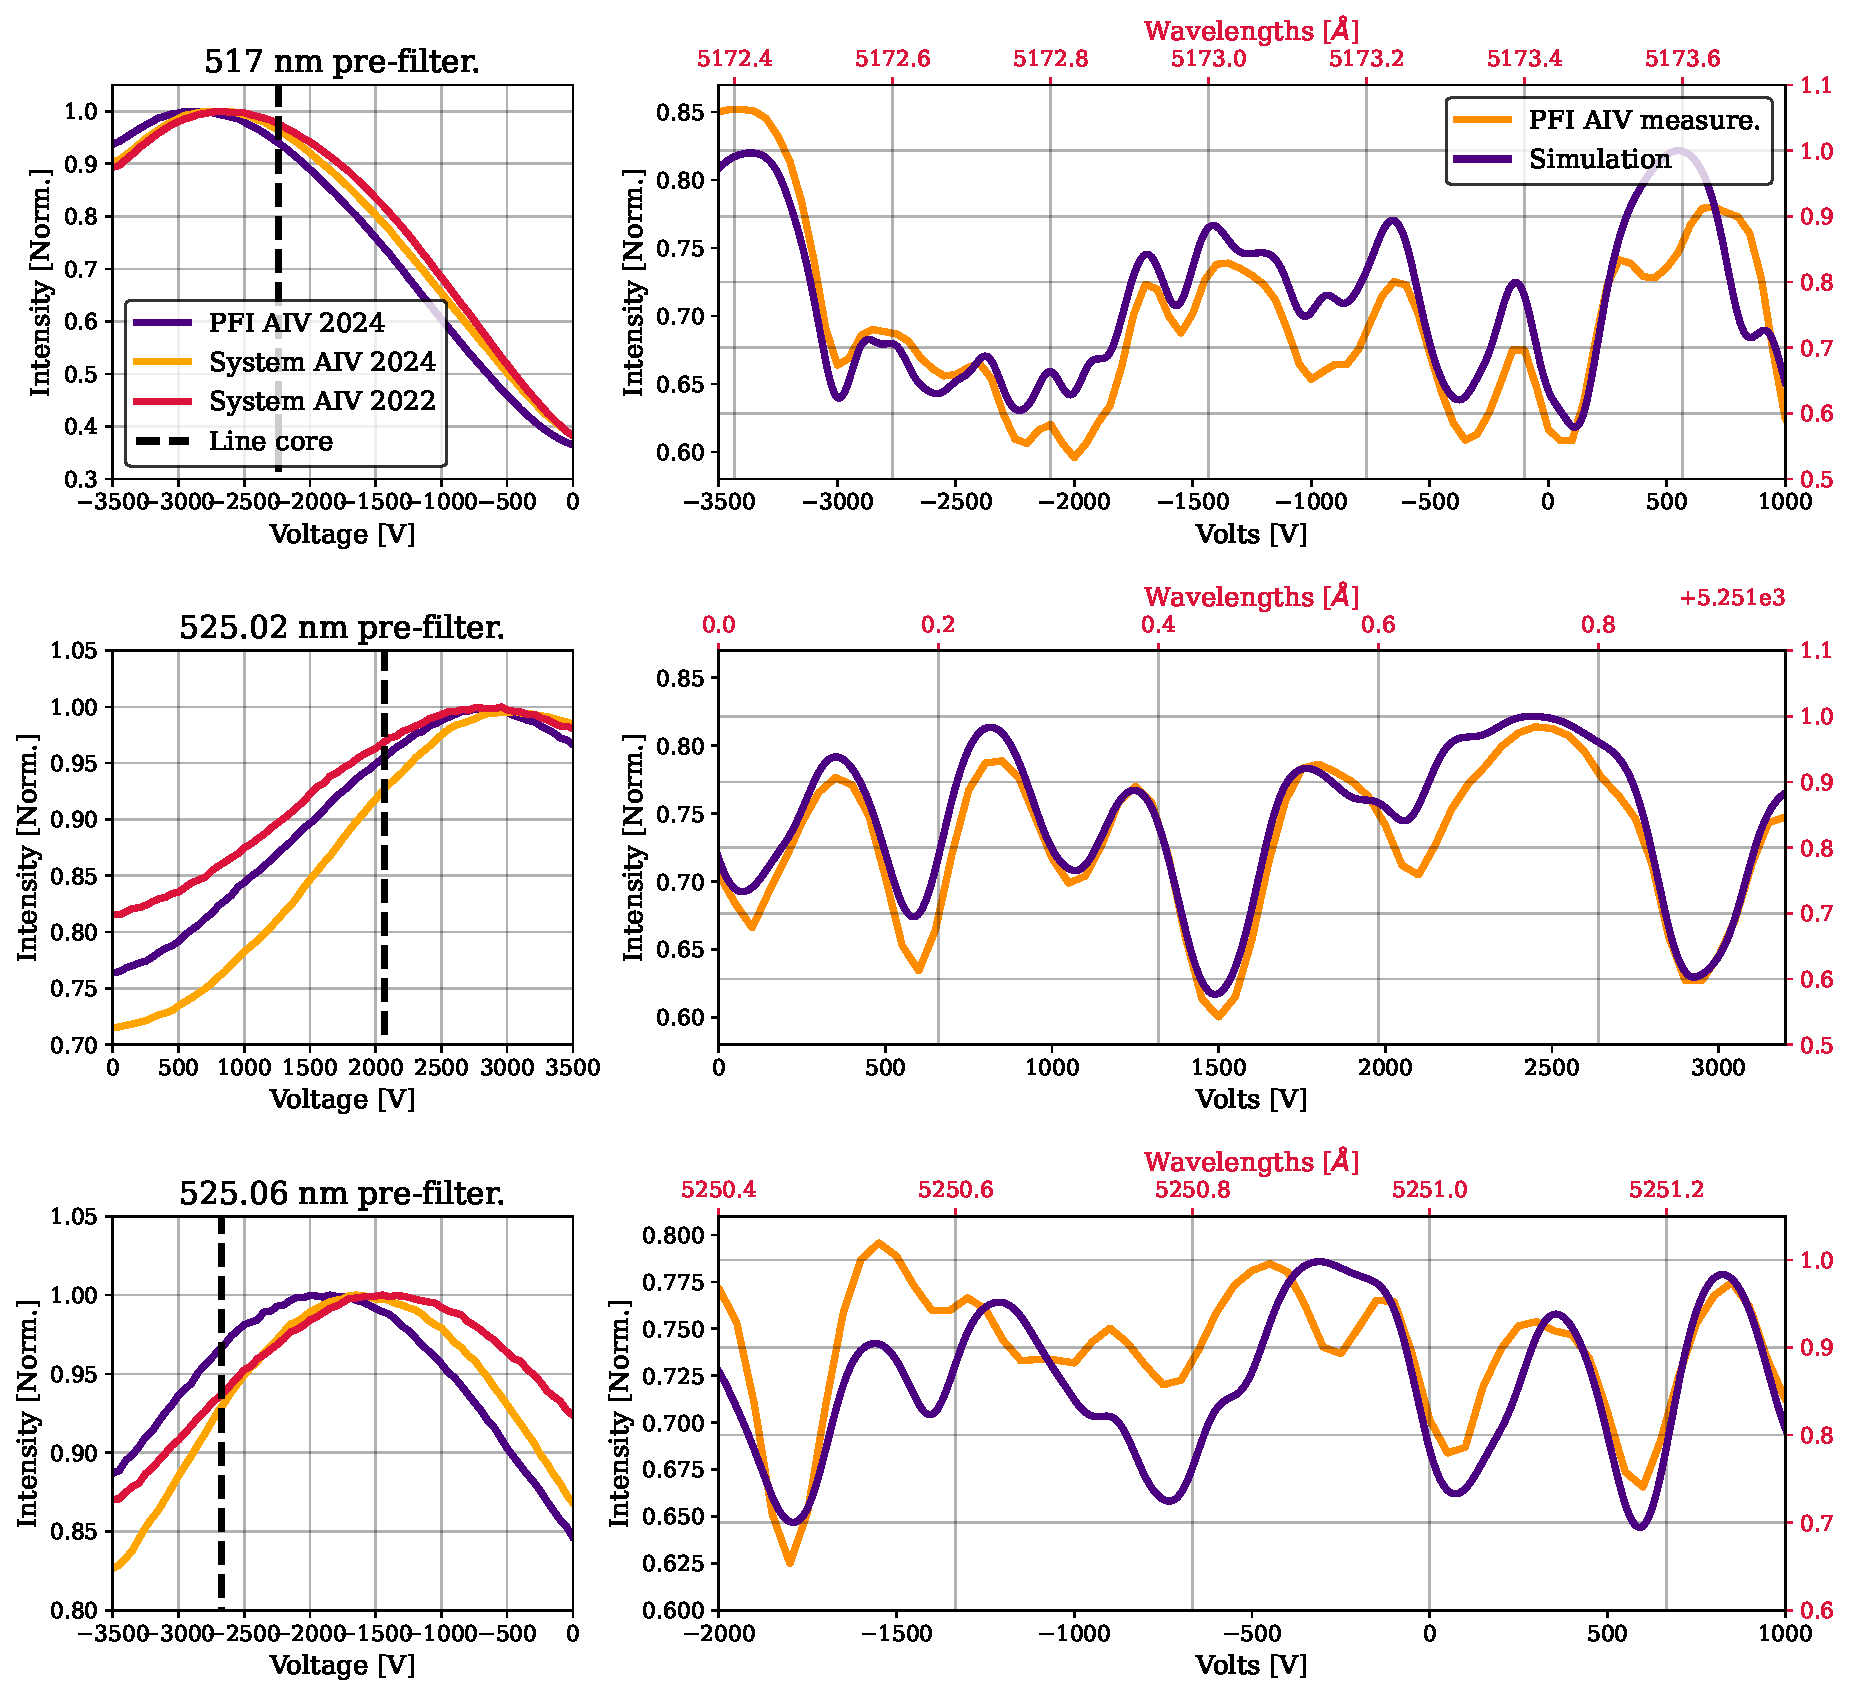
\includegraphics[width=\textwidth]{figures/TuMag/Spectroscopic_calibration.pdf}
    \caption{
      TuMag spectroscopic calibration results. Each row shows results for the 517 nm, 525.02 nm and 525.06 nm pre-filters, from top to row. The left column shows measurements of the pre-filters carried out with a flat LED on different stages of the AIV phases. The right column shows the fit of the I$_2$ cell observation with a simulation employing an etalon with a reflectivity of 0.892 (FWHM$\sim 0.87$). Note that the absolute value of the wavelengths of the simulation (red axis) might be shifted with respect to real values due to unknown conditions of the reference.   
      \label{fig_tumag: spectroscopic_results}}
\end{figure}

TuMag's etalon (see Table \ref{table: Tumags etalon}) operates in a collimated setup with a transmission profile with a FWHM of 0.87 pm (in the double-passs configuration), thus achieving a spectral resolution that exceeds the required 9 pm. Observations of an iodine cell illuminated with a diode were conducted to verify the transmission profile's shape and accurately assess the tuning constant. The right column of Fig.~\ref{fig_tumag: spectroscopic_results} presents, in orange, the iodine cell measurements obtained during the assembly, integration, and verification (AIV) phase of TuMag's integration into the Post Focal Instruments (PFI) platform, which took place at the Max Planck Institute for Solar System Research (MPS) in Göttingen, Germany, in November 2023. Additionally, the dark blue line in the figure represents a simulation of the iodine spectrum observations. This simulation was generated using an analytical model of the transmission profile of collimated etalons (see section \ref{susec_etalon_theory: collimated} for a detailed overview of the model). The results confirm that the spectral resolution achieved in the iodine cell observations is consistent with the estimated 0.87 pm resolution. Furthermore, these observations enabled the calculation of the etalon's tuning constant by identifying the corresponding line cores between the simulation and observation and applying a least squares fitting to establish the relationship, which was measured in 3300 V/\r{A}.

\begin{figure}[t]
    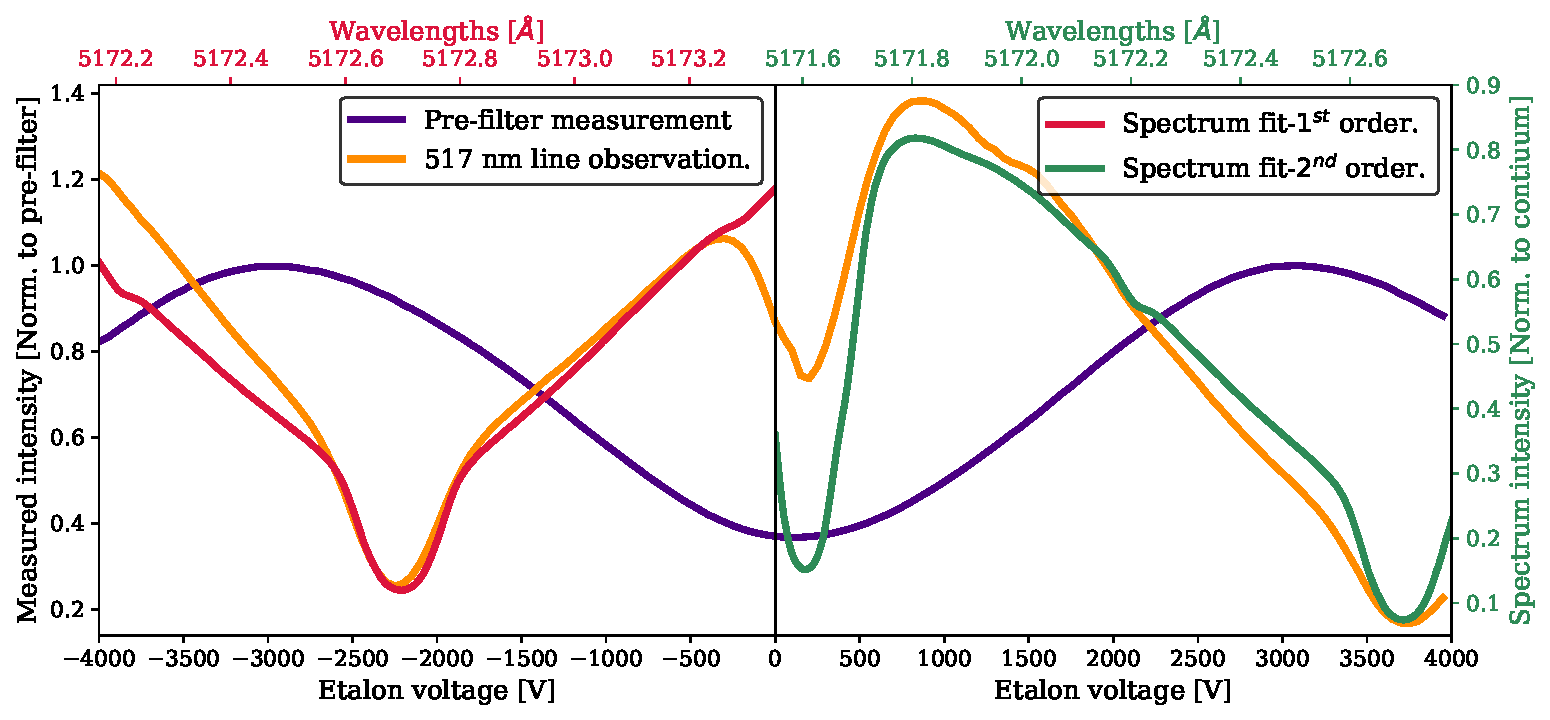
\includegraphics[width=\textwidth]{figures/TuMag/secondorder.pdf}
    \caption{
      Results of the spectroscopic calibration during the end-to-end calbrations of the AIV phase of 2021. The dark blue curve represents the measurement of the 517 nm pre-filter, alongside an observation of the magnesium line using the coelostat at INTA facilities, shown in orange. Two different fits of the solar spectrum are overplotted on the figure. The red line represents a fit to the primary etalon order (negtive voltages), while the green line corresponds to a fit to the second etalon order (positive voltages).      
      \label{fig_tumag:second-order_cont}}
\end{figure}

An observation of the solar spectrum with the 517 nm pre-filter, conducted at INTA facilities in December 2021 during the end-to-end calibration tests, is presented in Fig.~\ref{fig_tumag:second-order_cont}, along with the corresponding pre-filter measurement. The magnesium line core is detected at approximately -2200 V using the primary order of the etalon and reappears around 3750 V with a secondary order. A fitting of the solar spectrum\footnote{Reference} is also shown for both orders. These results reveal significant contamination from the secondary order near the pre-filter's minimum transmittance. At around 0 volts, the observed spectrum (orange line) is a composite of contributions from both the primary (red line) and secondary (green line) orders. This contamination is particularly relevant for data processing, as continuum measurements of the magnesium line are typically conducted at -80 V. The broader profile of the magnesium line necessitates continuum measurements farther from the line core, making it more susceptible to this contamination. In contrast, the narrower iron lines do not require such extensive offsets for continuum measurements and are thus less affected.

\subsubsection{\label{sect:tumag_cal polarimetric}Polarimetric performance.}

TuMag modulates the incoming light through a PMP composed of two anti-parallel LCVRs. These devices can modify the phase retardance induced to the light that goes through them by changing the alignment of their molecules when subject to a voltage potential. Their advantages for airborne instruments lie in their lightweight and compact design, the low voltage required for operation ([$0 - 10$]V), and their efficiency in producing either four linearly independent modulation states for full-Stokes polarimetry or only two states for measuring the longitudinal component of the magnetic field through Stokes V. This versatility is a specific advantage of LCVRs, not found in quarter-waveplate-based PMPs \citep{pmp-advantages}.

\begin{table}
    \centering
   \begin{tabular}{cc|cccc|cc}
    \hline
    \hline
     & & \multicolumn{4}{c}{Vectorial} & \multicolumn{2}{|c}{Longitudinal}  \\
     Spectral lines & Modulation & I1 & I2 & I3 & I4 & I1 & I2 \\
    \hline
    525 \& 517 nm & LCVR1 retardance  & 225$^\circ$  & 225 & 315$^\circ$ & 315$^\circ$ & 180$^\circ$  & 180$^\circ$\\
    525 \& 517 nm  & LCVR2 retardance  & 234.74$^\circ$ & 125.26$^\circ$ & 54.74$^\circ$ & 305.26$^\circ$ & 90$^\circ$ & 270$^\circ$ \\
    \hline
    525 nm & LCVR1 voltage & 2.291 & 2.533 & 1.992 & 1.947 & 2.761 & 2.761 \\
     & LCVR2 voltage & 2.375 & 3.360 & 6.433 & 2.016 & 4.723 & 2.186 \\
    \hline
    517 nm & LCVR1 voltage & 2.343 & 2.580 & 2.031 & 1.972 & 2.797 & 2.797\\
     & LCVR2 voltage & 2.371 & 3.416 & 6.548 & 2.051 & 4.77 & 2.206\\
    \hline
    \hline
    \end{tabular}
    \caption{Tumag LCVR retardances and corresponding voltages for both modulation schemes and the three pre-filters. Note that a single value is provided for both iron pre-filters.}
    \label{table: polarimetric configs}
\end{table}

TuMag's polarimetric measurement approach is divided into the two modulation schemes already mentioned: vectorial and longitudinal. In the vectorial scheme, four linearly independent modulation states are generated in rapid succession by the PMP, enabling the calculation of the full Stokes vector. Conversely, the longitudinal approach generates only two modulation states, providing information on just two components. This modulation is designed to compute Stokes V by determining the quantities $I\pm V$.

\begin{figure}[t]
    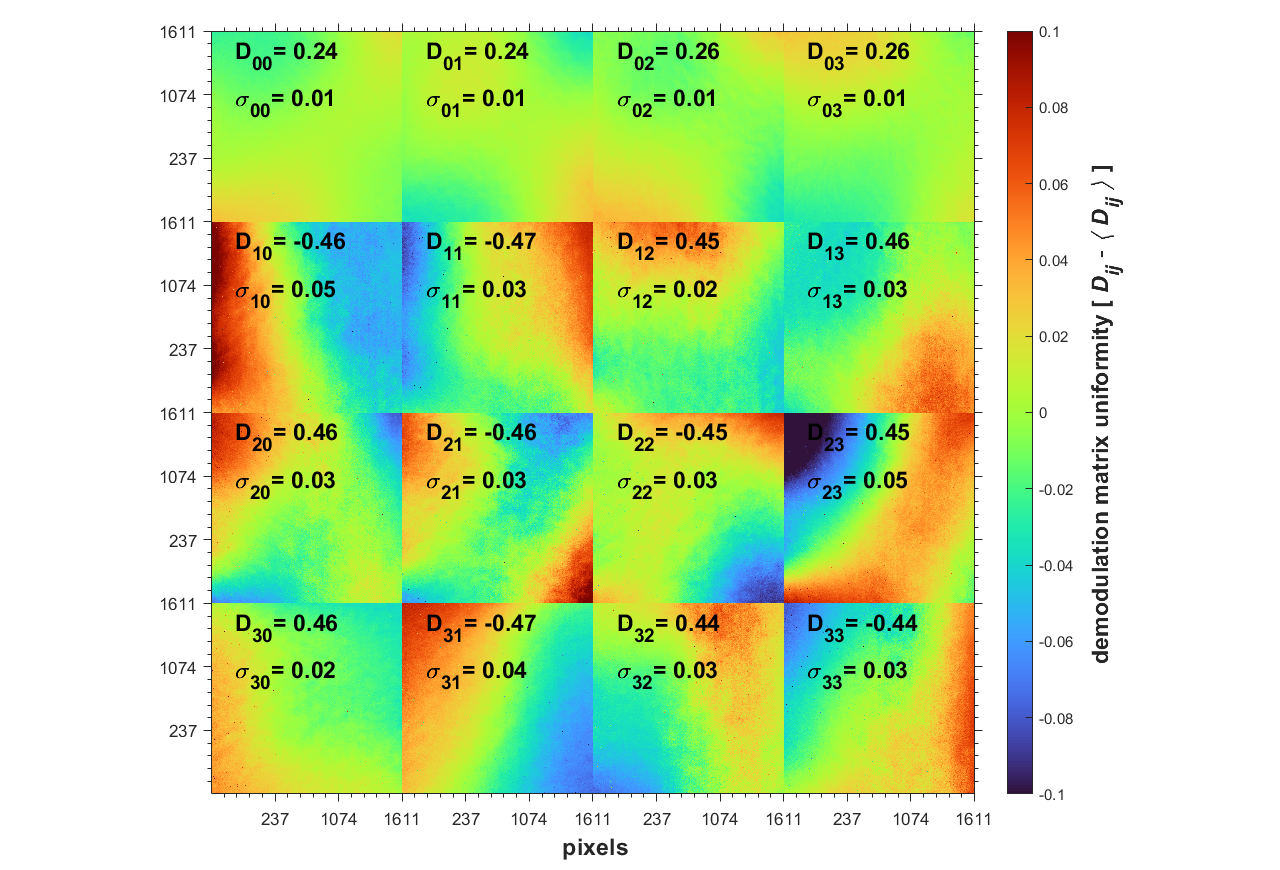
\includegraphics[width=\textwidth]{figures/TuMag/Pol_efficiencies_map.png}
    \caption{Polarimetric efficiencies for camera 1 and the three pre-filters (from top to bottom, the different rows show the results for 517 nm, 525.02 nm, and 525.06 nm). The different columns correspond to the efficiencies of the different Stokes components. The colormap measures the differences in efficiencies along the FoV. Results obtained during the E2E tests performed at INTA in December 2021, during the stand-alone AIV phase. 
    \label{fig_tumag:pol eff maps}}
\end{figure}

Both modulation schemes are required to operate under an optimal modulation scheme. Such a scheme is defined by a modulation matrix with the following polarimetric efficiencies: $\varepsilon _{opt} \geqslant [1, \frac{1}{\sqrt{3}}, \frac{1}{\sqrt{3}}, \frac{1}{\sqrt{3}}]$. The selected modulation scheme was based on the retardances outlined in Table \ref{table: polarimetric configs}. A thorough calibration of the liquid crystal variable retarders (LCVRs) was conducted to accurately determine the voltages necessary to produce the specified retardances \citep{fine-tunin}.

Considerations on the (S/N) are critical for ensuring the required polarimetric sensitivity. Achieving an S/N of $10^3$ in the Stokes measurements imposes a requirement of $S/N \approx 1200$  for each modulation measurement per camera. This calculation assumes near-optimal polarimetric performance, and takes into account the dual-beam polarimetry technique, which increases the S/N by a factor of $\sqrt{2}$ when combining data from the two cameras. A single shot of the cameras is insufficient to reach these S/N values, as the sensors do not have enough capacity in their electron wells. To address this, multiple exposures are captured and subsequently summed during each observation. This \textit{accumulation} strategy, extensively tested and employed in various polarimeters (e.g., \citealt{accs1}, \citealt{accs2}, \citealt{accs3}), has proven compatible with image reconstruction techniques \citep{accs-image1, accs-image2}. It allows for adjusting S/N levels depending on the scientific objectives of the observation, balancing between velocity and polarimetric sensitivity.

However, in order to fulfill the polarimetric sensitivity requirements, the modulation matrix of the instrument must be carefully addressed during the polarimetric calibrations. Any deviation in the computation of the modulation matrix, will introduce spurious signals in the polarization measurements, known as cross-talk. The polarimetric calibration involves a series of measurements using a light beam with a known polarization state, generated by a rotating linear polarizer and a rotating quarter-waveplate. By varying the positions of these two devices, 40 different input polarization states were produced and measured with three pre-filters. These measurements allowed for the precise determination of the modulation matrix by solving the system of equations \eqref{eq_intro:modultaion_eqs}, where the only unknown is the modulation matrix $\textbf{M}$, as both the measured modulation and the Stokes components of the incoming light are known. The modulation matrices for both cameras (indicated through the subindex) and all pre-filters that were determined through this process during the polarimetric E2E tests conducted at the Sunrise III AIV phase in Kiruna, Sweden, in 2022, are:
\[
\begin{matrix}
M_0 ^{517} = \begin{bmatrix}
            0.951 & -0.612 & 0.474 & 0.459 \\
            0.955 & -0.331 & -0.758 & -0.382 \\
            1.058 & 0.456 & 0.562 & -0.712 \\
            1.036 & 0.747 & -0.260 & 0.600
            \end{bmatrix}
& \quad
M_1 ^{517} = \begin{bmatrix}
            1.054 & 0.763 & -0.394 & -0.524 \\
            1.036 & 0.497 & 0.793 & 0.306 \\
            0.953 & -0.282 & -0.475 & 0.683 \\
            0.958 & -0.585 & 0.320 & -0.613
            \end{bmatrix}
\\ \\
M _ 0 ^{525.02} = \begin{bmatrix}
    0.954 & -0.694 & 0.406 & 0.414 \\
    0.969 & -0.390 & -0.803 & -0.368 \\
    1.042 & 0.418 & 0.495 & -0.705 \\
    1.035 & 0.710 & -0.266 & 0.612
    \end{bmatrix}
& \quad
M _ 1 ^{525.02} = \begin{bmatrix}
    1.059 & 0.771 & -0.449 & -0.433 \\
    1.024 & 0.449 & 0.723 & 0.335 \\
    0.965 & -0.344 & -0.543 & 0.650 \\
    0.953 & -0.606 & 0.191 & -0.641
    \end{bmatrix}
\\ \\
M _ 0 ^{525.06} = \begin{bmatrix}
    0.951 & -0.687 & 0.403 & 0.424 \\
    0.962 & -0.373 & -0.800 & -0.339 \\
    1.048 & 0.415 & 0.500 & -0.728 \\
    1.038 & 0.736 & -0.236 & 0.601
    \end{bmatrix}
& \quad
M _ 1 ^{525.06} = \begin{bmatrix}
    1.060 & 0.777 & -0.403 & -0.463 \\
    1.032 & 0.471 & 0.754 & 0.290 \\
    0.960 & -0.306 & -0.497 & 0.681 \\
    0.948 & -0.620 & 0.205 & -0.619
    \end{bmatrix}
\end{matrix}
\]

The results of the polarimetric calibration performed during the end-to-end (E2E) tests at INTA in December 2021 are presented in Fig.~\ref{fig_tumag:pol eff maps}. The figure shows the results for camera one; however, camera two demonstrated nearly identical efficiencies. The polarimetric efficiencies across the entire field of view (FoV) exceed the required thresholds $\varepsilon _{req} \geqslant [0.95, 0.45, 0.45, 0.45]$, and approach the optimal values. Furthermore, efficiency variations along the FoV are generally low, with standard deviations lower than 0.01. This hmogeneity of the polarimetric performance makes the data reduction easier as no special treatment is requiered for specific regions.  




